% Options for packages loaded elsewhere
\PassOptionsToPackage{unicode}{hyperref}
\PassOptionsToPackage{hyphens}{url}
%
\documentclass[
]{article}
\usepackage{amsmath,amssymb}
\usepackage{lmodern}
\usepackage{ifxetex,ifluatex}
\ifnum 0\ifxetex 1\fi\ifluatex 1\fi=0 % if pdftex
  \usepackage[T1]{fontenc}
  \usepackage[utf8]{inputenc}
  \usepackage{textcomp} % provide euro and other symbols
\else % if luatex or xetex
  \usepackage{unicode-math}
  \defaultfontfeatures{Scale=MatchLowercase}
  \defaultfontfeatures[\rmfamily]{Ligatures=TeX,Scale=1}
\fi
% Use upquote if available, for straight quotes in verbatim environments
\IfFileExists{upquote.sty}{\usepackage{upquote}}{}
\IfFileExists{microtype.sty}{% use microtype if available
  \usepackage[]{microtype}
  \UseMicrotypeSet[protrusion]{basicmath} % disable protrusion for tt fonts
}{}
\makeatletter
\@ifundefined{KOMAClassName}{% if non-KOMA class
  \IfFileExists{parskip.sty}{%
    \usepackage{parskip}
  }{% else
    \setlength{\parindent}{0pt}
    \setlength{\parskip}{6pt plus 2pt minus 1pt}}
}{% if KOMA class
  \KOMAoptions{parskip=half}}
\makeatother
\usepackage{xcolor}
\IfFileExists{xurl.sty}{\usepackage{xurl}}{} % add URL line breaks if available
\IfFileExists{bookmark.sty}{\usepackage{bookmark}}{\usepackage{hyperref}}
\hypersetup{
  hidelinks,
  pdfcreator={LaTeX via pandoc}}
\urlstyle{same} % disable monospaced font for URLs
\usepackage[margin=1in]{geometry}
\usepackage{color}
\usepackage{fancyvrb}
\newcommand{\VerbBar}{|}
\newcommand{\VERB}{\Verb[commandchars=\\\{\}]}
\DefineVerbatimEnvironment{Highlighting}{Verbatim}{commandchars=\\\{\}}
% Add ',fontsize=\small' for more characters per line
\usepackage{framed}
\definecolor{shadecolor}{RGB}{248,248,248}
\newenvironment{Shaded}{\begin{snugshade}}{\end{snugshade}}
\newcommand{\AlertTok}[1]{\textcolor[rgb]{0.94,0.16,0.16}{#1}}
\newcommand{\AnnotationTok}[1]{\textcolor[rgb]{0.56,0.35,0.01}{\textbf{\textit{#1}}}}
\newcommand{\AttributeTok}[1]{\textcolor[rgb]{0.77,0.63,0.00}{#1}}
\newcommand{\BaseNTok}[1]{\textcolor[rgb]{0.00,0.00,0.81}{#1}}
\newcommand{\BuiltInTok}[1]{#1}
\newcommand{\CharTok}[1]{\textcolor[rgb]{0.31,0.60,0.02}{#1}}
\newcommand{\CommentTok}[1]{\textcolor[rgb]{0.56,0.35,0.01}{\textit{#1}}}
\newcommand{\CommentVarTok}[1]{\textcolor[rgb]{0.56,0.35,0.01}{\textbf{\textit{#1}}}}
\newcommand{\ConstantTok}[1]{\textcolor[rgb]{0.00,0.00,0.00}{#1}}
\newcommand{\ControlFlowTok}[1]{\textcolor[rgb]{0.13,0.29,0.53}{\textbf{#1}}}
\newcommand{\DataTypeTok}[1]{\textcolor[rgb]{0.13,0.29,0.53}{#1}}
\newcommand{\DecValTok}[1]{\textcolor[rgb]{0.00,0.00,0.81}{#1}}
\newcommand{\DocumentationTok}[1]{\textcolor[rgb]{0.56,0.35,0.01}{\textbf{\textit{#1}}}}
\newcommand{\ErrorTok}[1]{\textcolor[rgb]{0.64,0.00,0.00}{\textbf{#1}}}
\newcommand{\ExtensionTok}[1]{#1}
\newcommand{\FloatTok}[1]{\textcolor[rgb]{0.00,0.00,0.81}{#1}}
\newcommand{\FunctionTok}[1]{\textcolor[rgb]{0.00,0.00,0.00}{#1}}
\newcommand{\ImportTok}[1]{#1}
\newcommand{\InformationTok}[1]{\textcolor[rgb]{0.56,0.35,0.01}{\textbf{\textit{#1}}}}
\newcommand{\KeywordTok}[1]{\textcolor[rgb]{0.13,0.29,0.53}{\textbf{#1}}}
\newcommand{\NormalTok}[1]{#1}
\newcommand{\OperatorTok}[1]{\textcolor[rgb]{0.81,0.36,0.00}{\textbf{#1}}}
\newcommand{\OtherTok}[1]{\textcolor[rgb]{0.56,0.35,0.01}{#1}}
\newcommand{\PreprocessorTok}[1]{\textcolor[rgb]{0.56,0.35,0.01}{\textit{#1}}}
\newcommand{\RegionMarkerTok}[1]{#1}
\newcommand{\SpecialCharTok}[1]{\textcolor[rgb]{0.00,0.00,0.00}{#1}}
\newcommand{\SpecialStringTok}[1]{\textcolor[rgb]{0.31,0.60,0.02}{#1}}
\newcommand{\StringTok}[1]{\textcolor[rgb]{0.31,0.60,0.02}{#1}}
\newcommand{\VariableTok}[1]{\textcolor[rgb]{0.00,0.00,0.00}{#1}}
\newcommand{\VerbatimStringTok}[1]{\textcolor[rgb]{0.31,0.60,0.02}{#1}}
\newcommand{\WarningTok}[1]{\textcolor[rgb]{0.56,0.35,0.01}{\textbf{\textit{#1}}}}
\usepackage{graphicx}
\makeatletter
\def\maxwidth{\ifdim\Gin@nat@width>\linewidth\linewidth\else\Gin@nat@width\fi}
\def\maxheight{\ifdim\Gin@nat@height>\textheight\textheight\else\Gin@nat@height\fi}
\makeatother
% Scale images if necessary, so that they will not overflow the page
% margins by default, and it is still possible to overwrite the defaults
% using explicit options in \includegraphics[width, height, ...]{}
\setkeys{Gin}{width=\maxwidth,height=\maxheight,keepaspectratio}
% Set default figure placement to htbp
\makeatletter
\def\fps@figure{htbp}
\makeatother
\setlength{\emergencystretch}{3em} % prevent overfull lines
\providecommand{\tightlist}{%
  \setlength{\itemsep}{0pt}\setlength{\parskip}{0pt}}
\setcounter{secnumdepth}{-\maxdimen} % remove section numbering
\ifluatex
  \usepackage{selnolig}  % disable illegal ligatures
\fi

\author{}
\date{\vspace{-2.5em}}

\begin{document}

\begin{Shaded}
\begin{Highlighting}[]
\FunctionTok{getwd}\NormalTok{()}
\end{Highlighting}
\end{Shaded}

\begin{verbatim}
## [1] "/Users/timoerdelt/Uni/masterthesis/evaluation"
\end{verbatim}

\begin{Shaded}
\begin{Highlighting}[]
\FunctionTok{library}\NormalTok{(readxl)}
\NormalTok{nasa\_tlx }\OtherTok{\textless{}{-}} \FunctionTok{read\_excel}\NormalTok{(}\StringTok{"./nasa\_tlx\_data.xlsx"}\NormalTok{)}
\CommentTok{\# View(nasa\_tlx)}

\FunctionTok{library}\NormalTok{(ggsci)}
\FunctionTok{library}\NormalTok{(ggthemes)}
\FunctionTok{library}\NormalTok{(ggplot2)}

\NormalTok{workload }\OtherTok{\textless{}{-}}\NormalTok{ nasa\_tlx}\SpecialCharTok{$}\NormalTok{Workload}
\NormalTok{control }\OtherTok{\textless{}{-}}\NormalTok{ nasa\_tlx}\SpecialCharTok{$}\StringTok{\textasciigrave{}}\AttributeTok{Sense of control}\StringTok{\textasciigrave{}}
\NormalTok{creativity }\OtherTok{\textless{}{-}}\NormalTok{ nasa\_tlx}\SpecialCharTok{$}\StringTok{\textasciigrave{}}\AttributeTok{Creativity Support Index}\StringTok{\textasciigrave{}}
\NormalTok{value }\OtherTok{\textless{}{-}} \FunctionTok{c}\NormalTok{(}\FunctionTok{mean}\NormalTok{(workload), }\FunctionTok{mean}\NormalTok{(control), }\FunctionTok{mean}\NormalTok{(creativity))}
\NormalTok{sd }\OtherTok{\textless{}{-}} \FunctionTok{c}\NormalTok{(}\FunctionTok{sd}\NormalTok{(workload), }\FunctionTok{sd}\NormalTok{(control), }\FunctionTok{sd}\NormalTok{(creativity))}
\NormalTok{name }\OtherTok{\textless{}{-}} \FunctionTok{c}\NormalTok{(}\StringTok{"Workload"}\NormalTok{, }\StringTok{"Sense of control"}\NormalTok{, }\StringTok{"Creativity Support Index"}\NormalTok{)}

\NormalTok{data }\OtherTok{\textless{}{-}} \FunctionTok{data.frame}\NormalTok{(name, value, sd)}
\NormalTok{nasa\_tlx\_plot }\OtherTok{\textless{}{-}} \FunctionTok{ggplot}\NormalTok{(data, }\FunctionTok{aes}\NormalTok{(}\AttributeTok{fill=}\NormalTok{name, }\AttributeTok{x=}\FunctionTok{factor}\NormalTok{(name, }\AttributeTok{level=}\NormalTok{name), }\AttributeTok{y=}\NormalTok{value)) }\SpecialCharTok{+} 
  \FunctionTok{geom\_bar}\NormalTok{(}\AttributeTok{position=}\StringTok{"dodge"}\NormalTok{, }\AttributeTok{stat=}\StringTok{"identity"}\NormalTok{, }\AttributeTok{colour =} \StringTok{"\#000000"}\NormalTok{) }\SpecialCharTok{+} 
  \FunctionTok{geom\_errorbar}\NormalTok{(}\FunctionTok{aes}\NormalTok{(}\AttributeTok{x=}\NormalTok{name, }\AttributeTok{ymin=}\NormalTok{value}\SpecialCharTok{{-}}\NormalTok{sd, }\AttributeTok{ymax=}\NormalTok{value}\SpecialCharTok{+}\NormalTok{sd), }\AttributeTok{width=}\FloatTok{0.2}\NormalTok{) }\SpecialCharTok{+} 
  \FunctionTok{scale\_y\_continuous}\NormalTok{(}\AttributeTok{breaks =} \FunctionTok{c}\NormalTok{(}\DecValTok{0}\NormalTok{, }\DecValTok{20}\NormalTok{, }\DecValTok{40}\NormalTok{, }\DecValTok{60}\NormalTok{, }\DecValTok{80}\NormalTok{, }\DecValTok{100}\NormalTok{), }\AttributeTok{limits=}\FunctionTok{c}\NormalTok{(}\DecValTok{0}\NormalTok{,}\DecValTok{100}\NormalTok{)) }\SpecialCharTok{+}
  \FunctionTok{xlab}\NormalTok{(}\StringTok{" "}\NormalTok{) }\SpecialCharTok{+} \FunctionTok{ylab}\NormalTok{(}\StringTok{"Mean"}\NormalTok{) }\SpecialCharTok{+}
  \FunctionTok{guides}\NormalTok{(}\AttributeTok{fill=}\StringTok{"none"}\NormalTok{) }\SpecialCharTok{+}
  \FunctionTok{theme\_minimal}\NormalTok{() }\SpecialCharTok{+}
  \FunctionTok{scale\_fill\_brewer}\NormalTok{(}\AttributeTok{palette =} \StringTok{"Blues"}\NormalTok{)}\SpecialCharTok{+}
  \FunctionTok{theme}\NormalTok{(}\AttributeTok{legend.position=}\StringTok{"bottom"}\NormalTok{)}

\FunctionTok{print}\NormalTok{(nasa\_tlx\_plot)}
\end{Highlighting}
\end{Shaded}

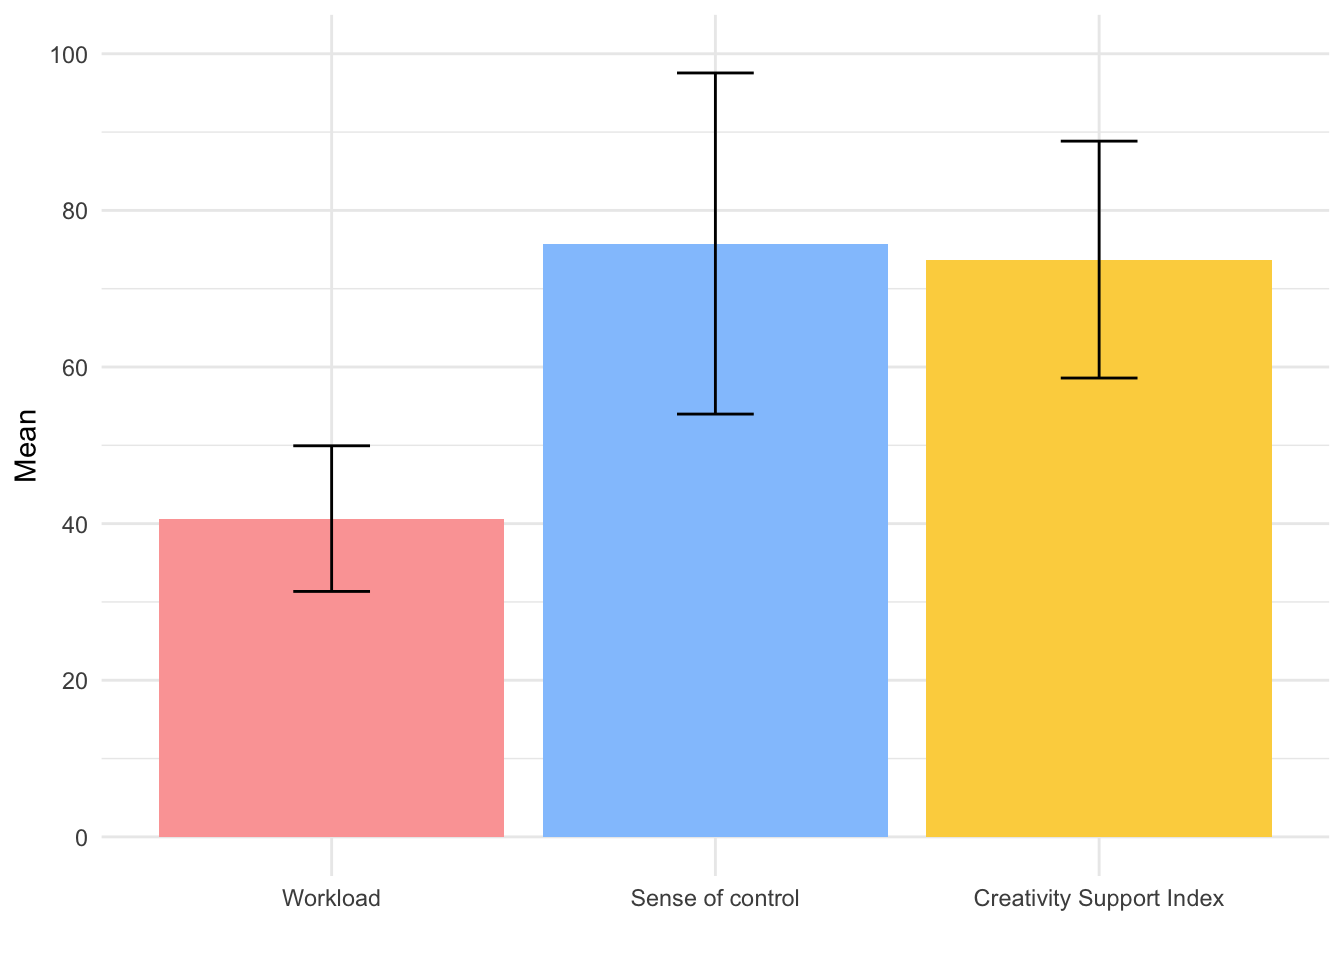
\includegraphics{evaluation_files/figure-latex/unnamed-chunk-1-1.pdf}

\begin{Shaded}
\begin{Highlighting}[]
\FunctionTok{ggsave}\NormalTok{(}\StringTok{"nasa\_tlx\_plot.eps"}\NormalTok{,}
       \AttributeTok{plot =}\NormalTok{ nasa\_tlx\_plot,}
       \AttributeTok{device =} \StringTok{"eps"}\NormalTok{,}
       \AttributeTok{scale =} \DecValTok{1}\NormalTok{, }\AttributeTok{units =} \StringTok{"cm"}\NormalTok{,}
       \AttributeTok{dpi =} \DecValTok{300}\NormalTok{,}
       \AttributeTok{limitsize =} \ConstantTok{TRUE}\NormalTok{)}
\end{Highlighting}
\end{Shaded}

\begin{verbatim}
## Saving 16.5 x 11.4 cm image
\end{verbatim}

\begin{Shaded}
\begin{Highlighting}[]
\FunctionTok{getwd}\NormalTok{()}
\end{Highlighting}
\end{Shaded}

\begin{verbatim}
## [1] "/Users/timoerdelt/Uni/masterthesis/evaluation"
\end{verbatim}

\begin{Shaded}
\begin{Highlighting}[]
\FunctionTok{library}\NormalTok{(readxl)}

\FunctionTok{library}\NormalTok{(ggsci)}
\FunctionTok{library}\NormalTok{(ggthemes)}
\FunctionTok{library}\NormalTok{(ggplot2)}
\FunctionTok{library}\NormalTok{(reshape2)}
\FunctionTok{library}\NormalTok{(gridExtra)}

\NormalTok{diff\_h }\OtherTok{\textless{}{-}} \FunctionTok{read\_excel}\NormalTok{(}\StringTok{"./Diff.xlsx"}\NormalTok{, }\AttributeTok{sheet =} \StringTok{"diff\_h"}\NormalTok{)}
\NormalTok{diff\_due }\OtherTok{\textless{}{-}} \FunctionTok{read\_excel}\NormalTok{(}\StringTok{"./Diff.xlsx"}\NormalTok{, }\AttributeTok{sheet =} \StringTok{"diff\_due"}\NormalTok{)}
\NormalTok{diff\_order }\OtherTok{\textless{}{-}} \FunctionTok{read\_excel}\NormalTok{(}\StringTok{"./Diff.xlsx"}\NormalTok{, }\AttributeTok{sheet =} \StringTok{"diff\_order"}\NormalTok{)}

\NormalTok{data\_h }\OtherTok{\textless{}{-}} \FunctionTok{melt}\NormalTok{(diff\_h, }\AttributeTok{id.vars=}\FunctionTok{c}\NormalTok{(}\StringTok{"Participant ID"}\NormalTok{, }\StringTok{"Type"}\NormalTok{))}
\NormalTok{data\_due }\OtherTok{\textless{}{-}} \FunctionTok{melt}\NormalTok{(diff\_due, }\AttributeTok{id.vars=}\FunctionTok{c}\NormalTok{(}\StringTok{"Participant ID"}\NormalTok{, }\StringTok{"Type"}\NormalTok{))}
\NormalTok{data\_order }\OtherTok{\textless{}{-}} \FunctionTok{melt}\NormalTok{(diff\_order, }\AttributeTok{id.vars=}\FunctionTok{c}\NormalTok{(}\StringTok{"Participant ID"}\NormalTok{))}

\NormalTok{plot\_h }\OtherTok{\textless{}{-}} \FunctionTok{ggplot}\NormalTok{(data\_h, }\FunctionTok{aes}\NormalTok{(}\AttributeTok{x=}\NormalTok{Type, }\AttributeTok{y=}\NormalTok{value, }\AttributeTok{fill=}\NormalTok{variable)) }\SpecialCharTok{+} 
  \FunctionTok{geom\_boxplot}\NormalTok{() }\SpecialCharTok{+} 
  \CommentTok{\# geom\_jitter() +}
  \FunctionTok{xlab}\NormalTok{(}\StringTok{" "}\NormalTok{) }\SpecialCharTok{+} \FunctionTok{ylab}\NormalTok{(}\StringTok{"Difference finish date in hours"}\NormalTok{) }\SpecialCharTok{+} 
  \FunctionTok{theme\_minimal}\NormalTok{() }\SpecialCharTok{+} 
  \FunctionTok{theme}\NormalTok{(}\AttributeTok{legend.title =} \FunctionTok{element\_blank}\NormalTok{()) }\SpecialCharTok{+}
  \FunctionTok{scale\_fill\_brewer}\NormalTok{(}\AttributeTok{palette =} \StringTok{"Blues"}\NormalTok{)}

\NormalTok{plot\_due }\OtherTok{\textless{}{-}} \FunctionTok{ggplot}\NormalTok{(data\_due, }\FunctionTok{aes}\NormalTok{(}\AttributeTok{x=}\NormalTok{Type, }\AttributeTok{y=}\NormalTok{value, }\AttributeTok{fill=}\NormalTok{variable)) }\SpecialCharTok{+} 
  \FunctionTok{geom\_boxplot}\NormalTok{() }\SpecialCharTok{+} 
  \CommentTok{\# geom\_jitter() +}
  \FunctionTok{xlab}\NormalTok{(}\StringTok{" "}\NormalTok{) }\SpecialCharTok{+} \FunctionTok{ylab}\NormalTok{(}\StringTok{"Difference due dates missed"}\NormalTok{) }\SpecialCharTok{+}
  \FunctionTok{theme\_minimal}\NormalTok{() }\SpecialCharTok{+} 
  \FunctionTok{theme}\NormalTok{(}\AttributeTok{legend.title =} \FunctionTok{element\_blank}\NormalTok{()) }\SpecialCharTok{+}
  \FunctionTok{scale\_fill\_brewer}\NormalTok{(}\AttributeTok{palette =} \StringTok{"Blues"}\NormalTok{)}

\NormalTok{plot\_order }\OtherTok{\textless{}{-}} \FunctionTok{ggplot}\NormalTok{(}\FunctionTok{melt}\NormalTok{(diff\_order, }\AttributeTok{id.vars=}\FunctionTok{c}\NormalTok{(}\StringTok{"Participant ID"}\NormalTok{)), }\FunctionTok{aes}\NormalTok{(}\AttributeTok{x=}\NormalTok{variable, }\AttributeTok{y=}\NormalTok{value, }\AttributeTok{fill=}\NormalTok{variable)) }\SpecialCharTok{+} 
  \FunctionTok{geom\_boxplot}\NormalTok{() }\SpecialCharTok{+} 
  \CommentTok{\# geom\_jitter() +}
  \FunctionTok{xlab}\NormalTok{(}\StringTok{" "}\NormalTok{) }\SpecialCharTok{+} \FunctionTok{ylab}\NormalTok{(}\StringTok{"Similarity to proposed order"}\NormalTok{) }\SpecialCharTok{+} 
  \FunctionTok{guides}\NormalTok{(}\AttributeTok{fill=}\StringTok{"none"}\NormalTok{) }\SpecialCharTok{+}
  \FunctionTok{theme\_minimal}\NormalTok{() }\SpecialCharTok{+} 
  \FunctionTok{scale\_fill\_brewer}\NormalTok{(}\AttributeTok{palette =} \StringTok{"Blues"}\NormalTok{)}

\NormalTok{plot\_h}
\end{Highlighting}
\end{Shaded}

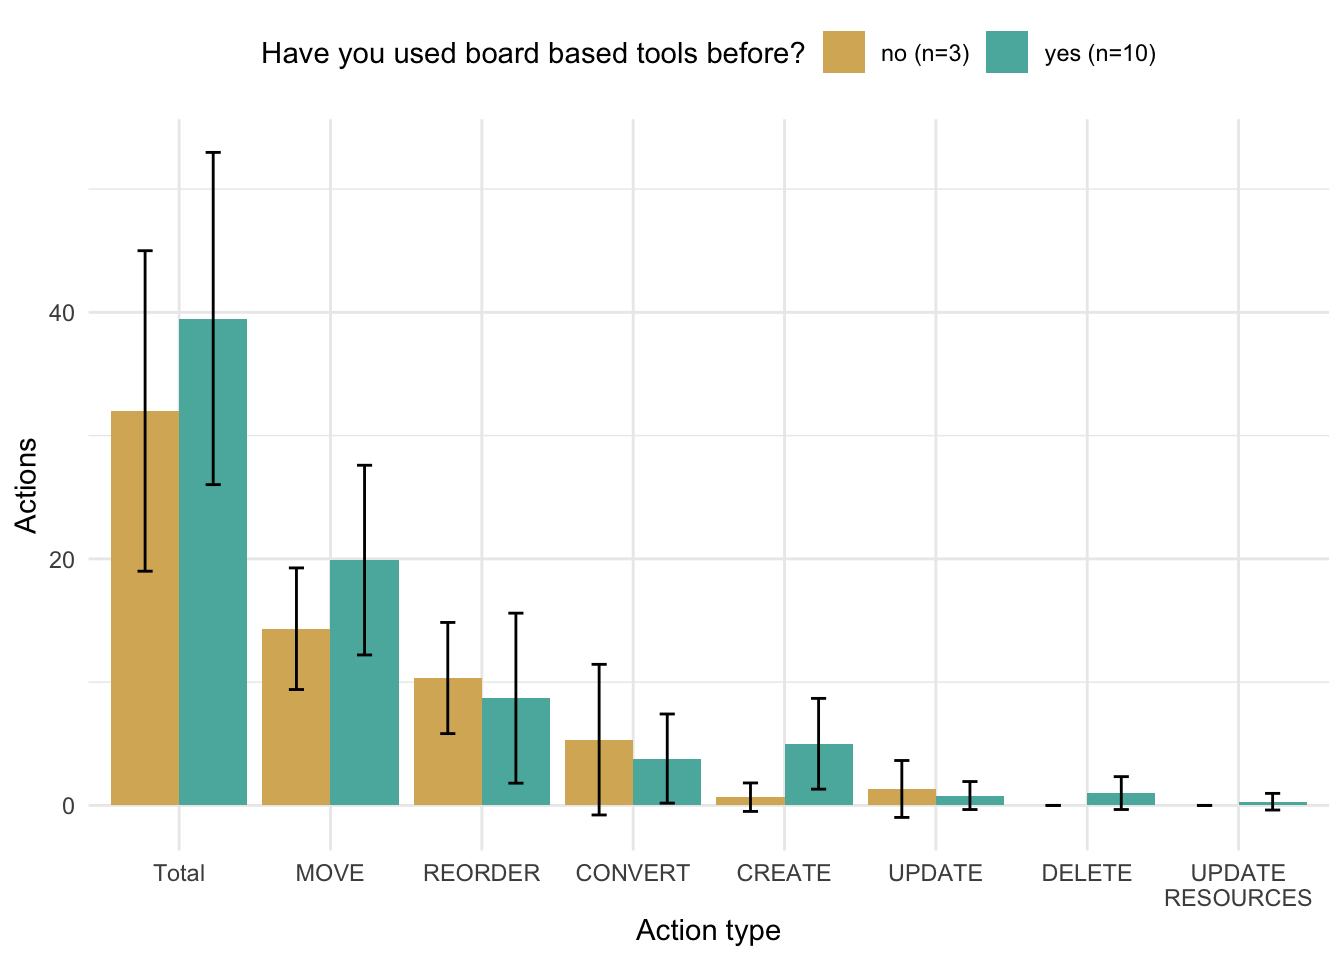
\includegraphics{evaluation_files/figure-latex/unnamed-chunk-2-1.pdf}

\begin{Shaded}
\begin{Highlighting}[]
\NormalTok{plot\_due}
\end{Highlighting}
\end{Shaded}

\includegraphics{evaluation_files/figure-latex/unnamed-chunk-2-2.pdf}

\begin{Shaded}
\begin{Highlighting}[]
\NormalTok{plot\_order}
\end{Highlighting}
\end{Shaded}

\includegraphics{evaluation_files/figure-latex/unnamed-chunk-2-3.pdf}

\begin{Shaded}
\begin{Highlighting}[]
\FunctionTok{ggsave}\NormalTok{(}\StringTok{"diff\_h.eps"}\NormalTok{,}
       \AttributeTok{plot =}\NormalTok{ plot\_h,}
       \AttributeTok{device =} \StringTok{"eps"}\NormalTok{,}
       \AttributeTok{scale =} \DecValTok{1}\NormalTok{, }\AttributeTok{units =} \StringTok{"cm"}\NormalTok{,}
       \AttributeTok{dpi =} \DecValTok{300}\NormalTok{,}
       \AttributeTok{limitsize =} \ConstantTok{TRUE}\NormalTok{)}
\end{Highlighting}
\end{Shaded}

\begin{verbatim}
## Saving 16.5 x 11.4 cm image
\end{verbatim}

\begin{Shaded}
\begin{Highlighting}[]
\FunctionTok{ggsave}\NormalTok{(}\StringTok{"diff\_due.eps"}\NormalTok{,}
       \AttributeTok{plot =}\NormalTok{ plot\_due,}
       \AttributeTok{device =} \StringTok{"eps"}\NormalTok{,}
       \AttributeTok{scale =} \DecValTok{1}\NormalTok{, }\AttributeTok{units =} \StringTok{"cm"}\NormalTok{,}
       \AttributeTok{dpi =} \DecValTok{300}\NormalTok{,}
       \AttributeTok{limitsize =} \ConstantTok{TRUE}\NormalTok{)}
\end{Highlighting}
\end{Shaded}

\begin{verbatim}
## Saving 16.5 x 11.4 cm image
\end{verbatim}

\begin{Shaded}
\begin{Highlighting}[]
\FunctionTok{ggsave}\NormalTok{(}\StringTok{"diff\_order.eps"}\NormalTok{,}
       \AttributeTok{plot =}\NormalTok{ plot\_order,}
       \AttributeTok{device =} \StringTok{"eps"}\NormalTok{,}
       \AttributeTok{scale =} \DecValTok{1}\NormalTok{, }\AttributeTok{units =} \StringTok{"cm"}\NormalTok{,}
       \AttributeTok{dpi =} \DecValTok{300}\NormalTok{,}
       \AttributeTok{limitsize =} \ConstantTok{TRUE}\NormalTok{)}
\end{Highlighting}
\end{Shaded}

\begin{verbatim}
## Saving 16.5 x 11.4 cm image
\end{verbatim}

\end{document}
